\chapter{基于势能损失的隐私保护拆分学习}
\label{chap:peloss}
在拆分学习中,各方运算自身对应的部分模型并交换中间结果,从而实现多方的推断和训练。
%
虽然拆分学习过程中各方没有暴露原始的输入数据,但是其中间结果的交换也带来了隐私泄漏风险。
%
其中一个主要的风险是模型补全攻击(Model Completion Attack)~\cite{fucong2022label_infer_attack},即在分类任务中,攻击者可以很容易根据中间结果和少量泄露的标签训练出高准确率的顶部模型,从而实现窃取模型或标签信息的目的。
%
本文将模型补全攻击转化为攻击者的有监督或无监督学习问题,从泛化误差角度对其进行了分析,并由电磁学现象启发,提出了势能损失函数,对模型补全攻击实现了有效的防护。
%

\section{研究背景}
拆分学习是一种高效的隐私保护机器学习手段~\cite{vepakomma2018split,poirot2019split}。
在拆分学习中,模型被分割为数个部分分发给各个参与方,各个参与方在模型的训练或推断过程中只需要交换中间结果而非原始数据,在一定程度上保护了数据的和模型参数的隐私。
%
相比于基于密码学的隐私保护机器学习方法,拆分学习具有非常高的通讯和计算效率。
%
如今拆分学习已经被应用在机器学习的多个领域中~\cite{palanisamy2021spliteasy,fagbohungbe2022split_edge_image,ccc2022vfgnn}。

由于第\ref{chap:randomized_topk}章中已经对拆分学习进行了基本的介绍,本节对此不再赘述。
%
虽然拆分学习拥有实现简单、效率高等诸多优势,但是在训练和推断过程中,各方直接交换了中间结果和中间梯度的明文,从而存在一定的隐私泄漏风险。
%
本章主要考虑的是拆分学习中的模型和标签数据的隐私问题。
%
不失一般性地,我们考虑两方拆分学习的场景,其中用户拥有输入特征($X$),而模型拥有方拥有模型参数并把底部模型($M_b$)下发给用户。
一个两方拆分学习推断的流程可以表示为:
\begin{equation}
    X \stackrel{M_b}{\to} H \stackrel{M_t}{\to} Y,
\end{equation}
其中,$X$是输入特征,$H$是拆分层的隐层表征,$Y$是预测的样本标签,而$M_b, M_t$表示底部模型和顶部模型。
%
可以看出,拆分层表征$H$同输入特征$X$、预测值$Y$都具有一定的相关性,因此有一定的隐私泄露风险。


目前已经有一些研究考察了从拆分层表征逆推输入特征的攻击,并提出了对应的防御手段,如Vepakomma等人~\cite{vepakomma2020nopeek}提出了在训练过程中加入额外的基于距离相关性~\cite{szekely2007dcor}的损失函数$\text{Dcor}(H, X)$来减少表征中包含的输入信息,并取得了一定的效果。
%
而拆分层表征泄露标签隐私的问题则更为严重。
%
Fu等人~\cite{fucong2022label_infer_attack}提出通过少量泄漏的带标签样本即可从随机初始化训练出顶部模型,从而窃取样本的标签以及整体模型,并将这种攻击称之为模型补全攻击(Model Completion Attack)。
%
针对这种攻击,Sun等人~\cite{sunjiankai2022forward_embedding_protect}提出使用距离相关性对表征和输出标签进行解耦,并取得了一定的效果。
%
除此之外,拆分学习的训练过程中的梯度也会泄露标签隐私。
Li等人~\cite{oscarli2022label_defense_marvell}表明的拆分层的梯度和样本标签的相关性很高,并提出了一些对于二分类模型的防御方法。
Sanjay等人~\cite{sanjay2023exploit_split_learning}在训练时采用替代的头部模型对梯度进行匹配从而实现盗取标签的目的。
%
本文研究的是针对分类模型的拆分学习推断阶段,尽可能地对$H\to Y$这一隐私泄漏链条进行保护,防止模型补全攻击。

直觉而言,拆分层表征泄露模型输出信息似乎是不可避免的。
%
因为在模型训练过程中,其逐渐丢弃隐层表征中关于输入特征的无关信息,只保留与标签相关的信息。
为了模型能产生准确的预测,隐层表征中必须包含关于标签的信息。
%
因此,本文并不尝试将标签相关信息从拆分层表征中彻底删除,而是把攻击问题转化成一个监督学习或无监督学习问题,研究如何使得攻击者难以从拆分层表征中获取标签信息。
%

\section{问题描述}
本节我们对拆分学习中底部模型产生的拆分层表征带来的对顶部模型以及标签的隐私泄漏问题(模型补全攻击)进行描述和定义,并且将该隐私泄漏问题转化为一个攻击者的有监督或无监督的学习问题。

\begin{figure}[h!]
    \centering
    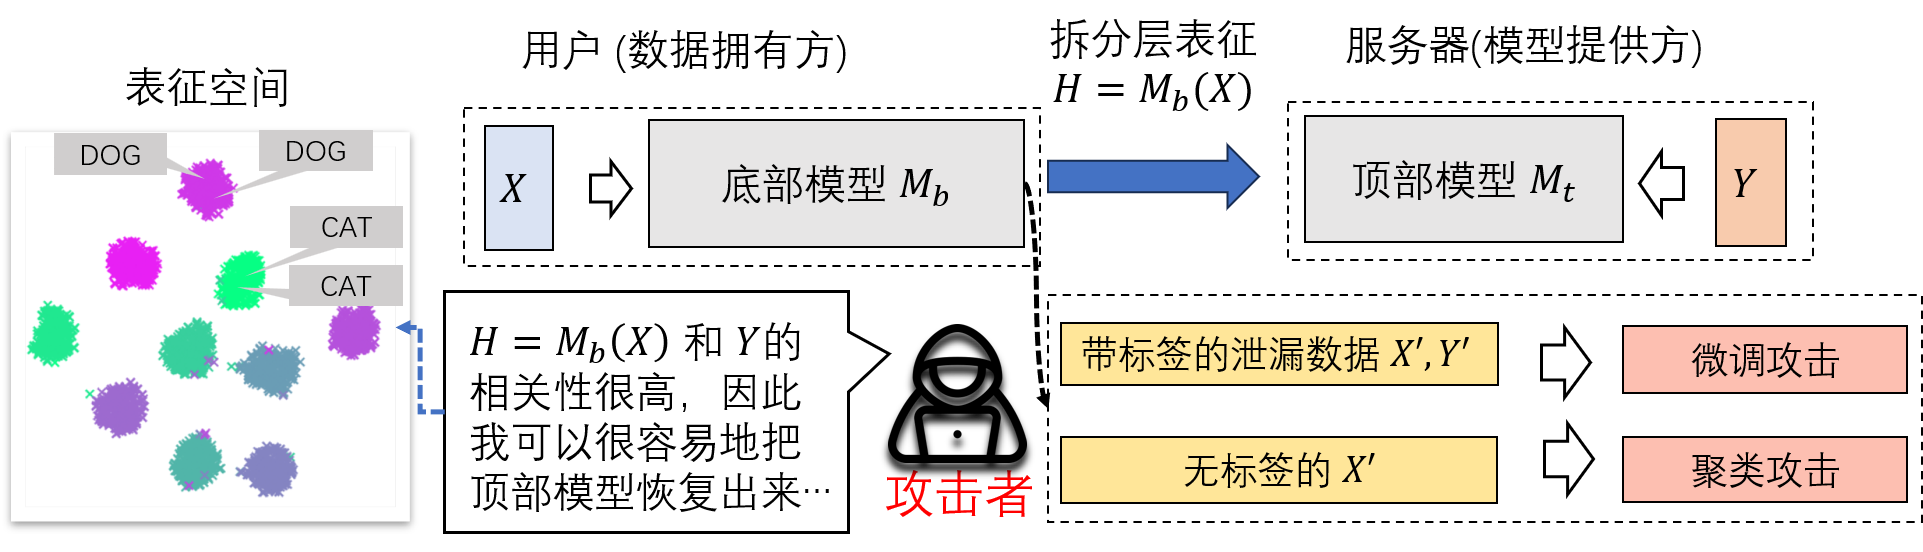
\includegraphics[width=1\linewidth]{Z_Resources/peloss_attack.png}
    \caption{拆分学习中底部模型带来的隐私泄露问题和模型补全攻击示意图}
    \label{fig:peloss:attack}
\end{figure}

\subsection{拆分层的隐私泄露}
许多对神经网络隐层进行可视化的研究都揭露了如下的规律:在神经网络的训练过程中,隐层表征与样本标签的关联性逐渐增加,相同标签对应的隐层表征会逐渐聚集成簇,而不同标签对应的隐层表征会逐渐分离开~\cite{paulo2017visualize_hidden,pezzotti2017deepeyes,cantareira2020hidden_vector_fields}。
%
并且位置越靠后(接近模型输出)的隐层的表征,与样本标签的关联性越高。
%
尽管上述的“同类别隐层表征靠近,不同类别隐层表征分离”的规律是神经网络具备学习能力的一个重要原因,这个规律也给拆分学习带来了很大的隐私泄漏风险。
%

理想的两方拆分学习$X \stackrel{M_b}{\to} H \stackrel{M_t}{\to} Y$应该满足下述的两个条件:
\begin{itemize}
    \item 从$H$推出$X$是困难的,从而保证用户的输入数据的隐私。
    \item 从$H$推出$Y$是困难的,因此用户必须和模型拥有方合作,才能获取模型预测值,而不能仅仅通过$M_b$获取预测值,从而保证模型的隐私。
\end{itemize}
然而,前面所述的神经网络隐层表征的性质,恰恰说明$H$推出$Y$可能是十分容易的,与我们期望的理想拆分学习的性质所矛盾。
%
假设攻击者腐化了用户,它可以轻松地通过少量带标签样本$(\cdots, (X_i, Y_i), \cdots)$,然后通过用户侧的底部模型$M_b$来产生拆分层表征$(\cdots, H_i, \cdots)$,并通过拆分层表征-标签对$(\cdots, (H_i, Y_i), \cdots)$来训练顶部模型$M_t$,从而窃取整个模型;
同时,攻击者也可以直接通过无标签的样本产生大量表征,并对其进行聚类得到类别标签,从而得到样本标签$Y$或训练出顶部模型$M_t$。
%
我们将这两种攻击统称为模型补全攻击,与现有研究一致~\cite{fucong2022label_infer_attack,liu2024vertical}。
%
\autoref{fig:peloss:attack}是模型补全攻击的示意图。


\subsection{威胁模型}
为了更清晰地定义上述的隐私泄漏问题,我们定义两种攻击方法:
\begin{itemize}
    \item \textbf{微调攻击}:
    假设攻击者具有底部模型$M_b$,并且拥有少部分泄露的带标签样本$Z = (\cdots, (X'_i, Y'_i), \cdots)$,其中每一种类别的样本都有$k$个。攻击者也知道顶部模型$M_t$的结构,但是不知道具体参数。
    攻击者通过泄漏样本$Z$和固定的$M_b$来微调(Fine-Tune)$M_t$,从而实现窃取模型的目的。

    \item \textbf{聚类攻击}:
    假设攻击者具有底部模型$M_b$,并且拥有大量泄漏的无标签样本$X = (\cdots, X_i, \cdots)$。
    攻击者通过$M_b$产生中间表征$H = (\cdots, H_i = M_b(X_i), \cdots)$,然后对其进行聚类产生类别标签,使得聚类模型实现顶部模型$M_t$的功能,从而窃取整个模型。
\end{itemize}

注意到,我们的攻击场景设定为拆分学习的推断阶段而非训练阶段,因为本文的目标是降低拆分层表征的隐私泄露。
%
如果要对拆分层梯度进行保护,可以使用非敏感数据进行训练,或者使用基于密码学的隐私保护神经网络训练方法~\cite{mohassel2017secureml,wagh2019securenn}。
%
除此之外,一些研究也指出对于无标签的样本进行无监督学习也能产生一个表现良好的分类模型~\cite{berthelot2019mixmatch,xuyi2021dp_ssl}。
但是这些方法与拆分学习无关,因为它们不需要任何关于底部模型或是拆分层表征的知识。
因此本文不考虑这些方法。
%

\subsection{问题定义}
表面上看来,上述的攻击和模型正常的训练过程的目标是类似的:两者都会学习从拆分层表征$H$到标签$Y$的映射。
%
然而攻击者的训练过程和正常的模型训练过程存在着一个本质区别,即两者的训练数据不同。
正常的模型训练过程需要大量的带标签数据,而在模型补全攻击中,我们假设攻击者只能获取少量的带标签样本(或是一定数量的无标签样本)。
%
因此,我们可以把模型补全攻击转化成一个机器学习问题,即攻击者使用少量带标签样本以及训练好的底部模型$M_b$来学习顶部模型$M_t$。
具体而言,防御的目标转换为:控制底部模型$M_b$,使得整体模型$(M_b, M_t)$有较高的准确率,但是使用少量带标签的$H = M_b(X)$对随机初始化的$M_t$进行微调,则会产生较高的泛化误差。
%

\begin{definition}[底部模型优势]
    我们定义底部模型优势为攻击者利用底部模型$M_b$进行攻击产生的额外优势。
    考虑一个攻击者$\mathcal A$和其输入数据$D$以及底部模型$M_b$(可以为空),其输出则为一个完整模型$M = (M_b, M_t): X \to Y$,底部模型优势可以定义为:
    \begin{equation}
        Adv(M_b; \mathcal A) = \mathbb E_D \{ R[\mathcal A(D; null)] - R[\mathcal A(D; M_b)]\},
    \end{equation}
    其中,$R[\cdot]$ 表示攻击者产生的完整模型在测试集上的误差,$\mathcal A(D; null)$ 表示攻击者在没有底部模型时的产生的完整模型。
\end{definition}
%
例如,在微调攻击时,$D = (\cdots, (X_i, Y_i), \cdots)$ 是泄露的带标签的样本;而在聚类攻击时,$D = (\cdots, X_i, \cdots)$是泄露的无标签的样本。
%
而$\mathcal A(D; null)$相当于攻击者在没有任何底部模型信息,仅有泄露数据的情况下产生的完整模型,即使用带标签数据/无标签数据从零开始训练模型(Train from Scratch)。

\begin{definition}[完美保护]
    对于某种攻击$\mathcal A$,如果底部模型$M_b$满足底部模型优势$Adv(M_b, \mathcal A) \le 0$,则称$M_b$对$\mathcal A$产生了完美保护,因为$M_b$的存在对攻击效果的提升没有任何作用。
\end{definition}

基于以上定义,本文目标可以描述为训练一个拆分学习模型$(M_b, M_t)$使得:
\begin{itemize}
    \item 模型本身的准确率越高越好。
    \item 微调攻击和聚类攻击的底部模型优势越小越好。
\end{itemize}
\section{势能损失函数}
如上节所述,我们把模型补全攻击考虑为攻击者基于泄露数据的机器学习过程。
%
本节我们研究攻击者在泄露样本上学习得到的顶部模型的泛化误差。
我们通过二分类例子表明当拆分层表征分布在决策边界附近时,攻击者的泛化误差较大。
%
受到静电平衡理论以及库仑定律的启发,我们提出了势能损失,使得拆分层表征满足上述的分布,从而实现对于模型补全攻击的保护。
%

\subsection{数据分布导致的学习误差}
我们从微调攻击的泛化误差以及聚类误差两个角度来说明同类样本分布在决策边界附近时可以使得攻击者的学习误差变大。


\subsubsection{泛化误差}
直观地说,当同类表征分布在决策边界附近时,表明同类表征之间的距离加大,从而使得少量该类别的表征无法代表整个类别的表征,因此会提高攻击者在少量样本上训练顶部模型的泛化误差。
%
下面我们使用一个二分类的例子对其进行说明。
%

考虑表征空间为一个$d$维超球体($d$-sphere)$\{ \bvec{x}: \sum_{i=1}^d x_i^2 = 1\}$,所有表征被划分为两个类别(正样本和负样本)。
令假设集(Hypothesis Set,即所有可能的分类函数的集合)为所有的半球面(表示正样本)集合:
\begin{equation}
    \mathcal H = \{ h: h(\bvec{x}) = \text{Sign}(\bvec{w} \cdot \bvec{x}), \Vert \bvec{w} \Vert_2 = 1\}.
\end{equation}
不失一般性,我们假设目标分类函数为$f(\bvec{x}) = \text{Sign}(x_1)$。
同时,我们对表征的分布做出如下假设:
\begin{itemize}
    \item 表征分布的概率密度仅仅和其坐标的第一维有关,也就是仅和$x_1$有关,而在其他维度上呈现出各向同性(Isotropic)性质。
    \item 给定一批正样本数据$S = \{\bvec{x}_1, \cdots, \bvec{x}_n\}$,学习算法简单地产生其归一化(Normalized)的平均值作为学到的分类模型的权重$\bvec{w}$。
    即:
    \begin{equation}
        f^{(S)}(\bvec{x}) = \text{Sign}\left[ \bvec{x} \cdot \sum_{i=1}^n {\bvec{x}_i} / \Vert \sum_{i=1}^n {\bvec{x}_i}\Vert_2 \right].
    \end{equation}
\end{itemize}

考虑当学习到的参数$\bvec{w} = \sum_{i=1}^n \bvec{x}_i / \Vert \sum_{i=1}^n \bvec{x}_i \Vert_2$ 与目标分类模型的参数 $\bvec{e}_1$ 有一个很小的偏差时的情况。
%
由于我们假设表征的分布在$\bvec{e}_1$之外的维度时各向同性的,我们可以假设$\bvec{w}$位于前两维展开的超平面上,也就是
\begin{equation}
    \bvec{w} = \bvec{e}_1 \cos \epsilon + \bvec{e}_2 \sin \epsilon,    
\end{equation}
其中$\epsilon$表示$\bvec{w}$和$\bvec{e}_1$之间的一个小角度。
%
此时我们可以得到泛化误差为:
\begin{equation}
\begin{split}
    1/2\cdot R[\bvec{w}] &= \mathop{\mathbb E}_{\bvec{x} \sim \mathcal S} \text{Sign}(x_1) \cdot I[x_1 \cos \epsilon + x_2 \sin \epsilon \le 0]
    \\
    & = \int_{\substack{x_1 > 0 \\ x_1 \cos \epsilon + x_2 \sin \epsilon \le 0 \\ x_1^2 + \cdots + x_d^2 = 1}} p(x_1, \cdots, x_d)dS
      \le \int_{\substack{x_1^2 + ... + x_d^2 = 1 \\0 < x_1 \le \tan\epsilon}}p(x_1, x_2, ...,x_d)dS
\end{split}
\end{equation}
注意到当$\epsilon \to 0$时,$\tan \epsilon \to \epsilon$,并且令$p_1$为表征在$\bvec{e}_1$上的边缘概率密度,即$p_1(x_1) = \int_{x_1^2 + \cdots + x_d^2} p(x_1, \cdots, x_d) dx_2\cdots dx_d$,
%
上式右侧可以进一步化为
\begin{equation}
    \int_{\substack{x_1^2 + ... + x_d^2 = 1 \\0 < x_1 \le \tan\epsilon}}p(x_1, x_2, ...,x_d)dS \approx \int_{x_1 = 0}^{\epsilon} p_1(x_1) dx_1 \approx \epsilon p_1(0).
\end{equation}
%
从上式可以看出,当$\epsilon$很小时,泛化误差的上界与$p_1(0)$呈近似线性关系。
由于$p_1(0)$就是正样本和负样本交界处的表征边缘概率密度,因此也可以说,此时泛化误差的大小与表征在决策边界附近的概率密度是成比例的。
越多的表征分布在决策边界上,则分类函数的(权重)误差导致的泛化误差就越大。

在上面的讨论中,我们假设$\epsilon$是一个固定的小量。
%
现在我们来讨论$\epsilon$与表征分布的关系。
%
对于任何一个随机变量$X$,如果$X_1, \cdots, X_m$是$m$个独立的采样,则有:
\begin{equation}
    \mathbb E \left[ \left(\dfrac{1}{m}\sum_{i=1}^m X_i - \mathbb E[X] \right)^2 \right] = \dfrac{1}{m} \mathbb E\left[\left(X -\mathbb EX\right)^2 \right].
\end{equation}
%
也就是说,如果随机变量的分布远离其均值,则多次采样后得到的采样均值相对于实际分布的均值的误差就越大。
%
虽然在先前的讨论中,我们假定表征空间是一个超球面,但是上述结论依然是近似成立的,也就是 $\mathbb E[\epsilon^2]\propto \mathbb E\left[(X - \mathbb EX)^2\right]$。
为了使得决策区域误差 $\epsilon$ 尽可能变大,同一类别的表征应该尽量分布在远离其分布均值的区域。
同时我们也可以注意到,离某一类别表征可以达到的距离分布均值最远的区域也正是该类别的决策边界。
%
上文的分析与从数据分布直接推导泛化误差上界的已有研究较为类似~\cite{jinpengzhan2020generalization},该研究使用数据的类内距离和类间距离对泛化误差上界进行估计。


%
\subsubsection{聚类误差}
当表征分布于决策边界附近时,对其进行聚类也将变得困难。
%
因为聚类的基本思想是把距离较近的一群数据点归入一个簇中~\cite{saxena2017cluster_review,murtagh_2012_cluster},也就是说,聚类之后的每个类别里面的数据点应该彼此靠近。
%
但是通过让表征分布到决策边界上,与其分布均值远离,同类表征之间的距离变得更大了,而不同类表征之间的距离变得更小了。
%
这与聚类的基本要求相违背,因此让表征分布于决策边界的做法很显然可以降低对其聚类的效果。


\subsubsection{总结}
综上所述,让表征分布到自身类别的决策边界,可以同时提高对其进行微调或聚类的学习误差,其原因可以总结为以下三点:
\begin{itemize}
    \item 学习得到的决策区域的误差$\epsilon$变大。
    \item 同样的决策区域误差$\epsilon$导致的模型泛化误差变大。
    \item 类间距离变小,类内距离变大。
\end{itemize}
我们将上述的分析直观地在\autoref{fig:peloss:method}中显示。

\begin{figure}[h!]
    \centering
    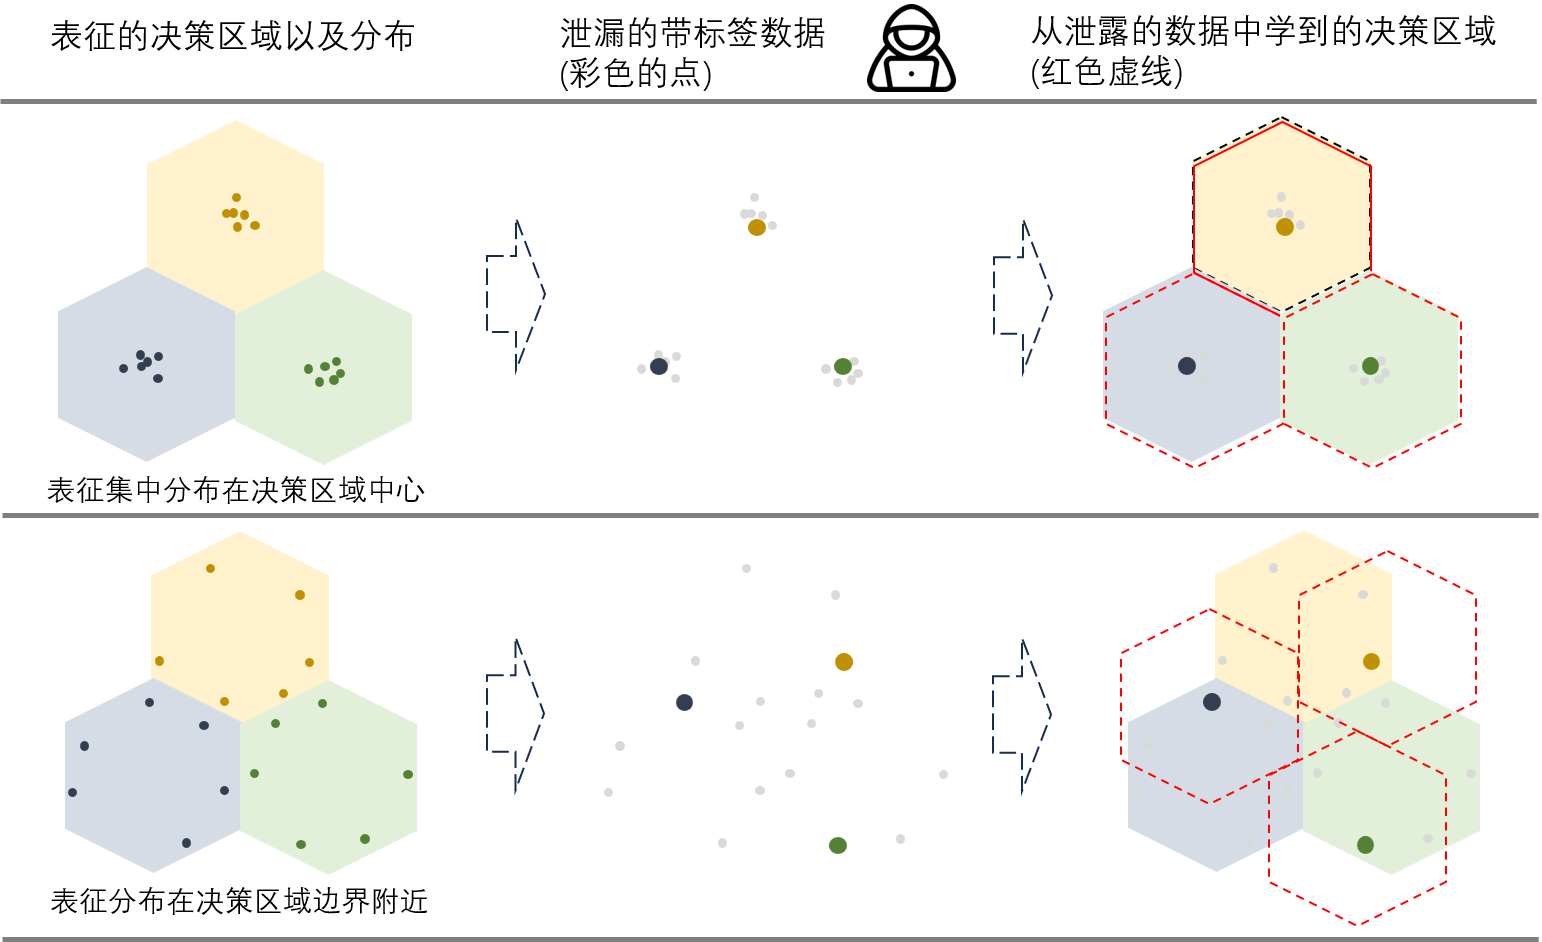
\includegraphics[width=1\linewidth]{Z_Resources/peloss_method.png}
    \caption{隐层表征分布导致的攻击者误差示意图}
    \label{fig:peloss:method}
\end{figure}


\subsection{势能损失函数定义}
物理学中的静电平衡(Electrostatic Equilibrium)现象告诉我们,当一个导体建立静电平衡时,其所有净电荷(Net Charge)将会分布在导体表面~\cite{griffiths2005introduction}。
%
这个现象的一部分原因时库仑定律(Coulomb's Law),即:同性电荷之间相互排斥,而异性电荷之间相互吸引。
%
受到该物理现象的启发,我们可以把相同类别的表征看作同性电荷,使得它们之间存在互相排斥对方的斥力。
因此,这些同类别的表征就会相互远离直到决策区域的边界处。
%

库仑定律的公式为
\begin{equation}
\label{eq:peloss:columb}
    \bvec{F} =  k {q_1q_2(\bvec{r}_1 - \bvec{r}_2)}/{\Vert r_1 - r_2 \Vert_2^3},
\end{equation}
其中,$k$表示一个常数,$q_1, q_2$是带符号的电荷大小(正电荷为正号,负电荷为负号),$\bvec{r}_1, \bvec{r}_2$表示两个电荷的位置,$\Vert \cdot \Vert$表示欧几里得范数,$\bvec{F}$则表示第二个电荷对第一个电荷产生的力(库仑力)的大小。
%
我们忽略常数以及电荷的大小,只考虑同性电荷,则可以把\autoref{eq:peloss:columb}化为$\bvec{F} = (\bvec{r}_1 - \bvec{r}_2) / \Vert\bvec{r}_1 - \bvec{r}_2 \Vert_2^3$。
%
由于库仑力也可以表示为电势能的梯度,我们可以进一步将其表示为梯度的形式$F = \nabla_{\bvec{r}_1} 1/\Vert \bvec{r}_1 - \bvec{r}_2 \Vert_2$。
%
这种表示方法与深度学习中所使用的梯度下降方法不谋而合。
%
基于以上分析,我们定义势能损失函数为:
\begin{equation}
    L_\text{pe} = \sum\limits_{c\in\mathcal C}\sum\limits_{\bvec{h} \in H_c}\sum\limits_{\bvec{h}' \in H_c, \bvec{h}' \ne \bvec{h}} \dfrac{1}{\Vert \bvec{h} - \bvec{h'} \Vert_2},
\end{equation}
其中$\mathcal C$表示标签的集合,$H_c$表示类别为$c$的表征集合。


通过把$L_{pe}$加入损失函数中,在拆分模型的训练过程中,同类别的表征互相之间会排斥并且逐渐移动到该类别的决策区域边界处。
%
在三维的情况下,汤姆森定理(Thomson's Theorem)证明电势能最小的情况对应于电荷全部分布在导体的表面~\cite{thomson_1913_atom,bakhoum_2008_thomson_proof},也就是此时表征的概率质量全部在决策边界。
%
但是考虑到拆分层的表征空间的维度一般远大于3维,因此其概率质量并不能完全集中在决策边界。
但是我们依然能证明,在势能损失函数最小的情况下,决策边界处必然有概率质量分布。

\begin{theorem}[决策边界的表征分布非零]
\label{thm:peloss:border-distribution}
    考虑一个$d$维有界区域$\Omega \subset \mathbb R^d$以及定义在$\Omega$内部的概率密度泛函$f^*$为最小化势能损失的概率密度:
    \begin{equation}
        \label{eq:peloss:potential-min}
        f^* = \mathop\textnormal{argmin}_f \textnormal{PE}(f) = \mathop\textnormal{argmin}_{f} \int_{\bvec{x} \in \Omega} \int_{y \in \Omega} \dfrac{f(\bvec{x})f(\bvec{y})}{\Vert \bvec{x} - \bvec{y} \Vert_2} dUdV,
    \end{equation}
    其中,$f$表示概率密度函数且满足$f \ge 0$(非负性) 以及 $\int_{\Omega} f(\bvec{x})dV = 1$(归一性)。
    令$\Delta_\epsilon \Omega = \{\bvec{x}: \bvec{x} + \epsilon \bvec{r} \not\in \Omega, \bvec{x} \in \Omega, \Vert \bvec{r} \Vert_2 = 1 \}$ 表示距离$\Omega$边界距离小于$\epsilon$的区域,那么$f^*$满足对于任意$\epsilon > 0$,有$\int_{\bvec{x}\in\Delta_\epsilon \Omega} f^*(\bvec{x})dV > 0$。
\end{theorem}
\begin{proof}
    为了让证明过程更加清晰,此处我们用$|\cdot |$来表示欧几里得范数。
    %
    首先考虑中心在$\bvec{x}_0$,半径为$r$的球$B_r(\bvec{x}_0)$。
    令
    \begin{equation}
        r_0 = \inf_r \left\{ \int_{\bvec{y}\in \Omega - B_{r}(\bvec{x}_0)} f(\bvec{y}) dV = 0 \right\},
    \end{equation}
    即:$f(x)$ 在$B_{r_0}(x_0)$ 之外几乎处处为0,也就是说$B_0 = B_{r_0}(x_0)$是以$x_0$为中心且包含了几乎所有概率质量的最小半径球。
    %
    因此我们可以找到一个靠近$B_0$边界的小球$B_1 = B_{\epsilon/4}(\bvec x_0 + \bvec{r}')$使得
    $\int_{\bvec{y}\in B_1} f(\bvec{y})dV = \delta$,其中$\delta > 0$,$|\bvec{r}'| = r_0 - \epsilon / 4$。
    也就是说,$B_1$内部的概率质量非零。
    %

    现在我们考虑将$f$在$B_1$里面的概率质量移动到$B_2 = B_{\epsilon/4}(\bvec x_0 + \bvec{r}'(1 + \dfrac{3\epsilon}{4|r'|})) = B_{\epsilon/4}(\bvec x_0 + \bvec{r}'')$中。
    %
    由于$B_2 \subset \Delta_\epsilon \Omega$且$B_1 \subset \Omega - \Delta_\epsilon \Omega$,所以上述的移动是可行的。
    %
    我们把概率质量移动后的概率密度函数记作
    \begin{equation}
        f'(\bvec{t}) = \begin{cases}
            f(\bvec{t} - \bvec{r}'' + \bvec{r}') & \quad \text{当 $\bvec{t} \in B_2$},\\
            0               & \quad \text{当 $\bvec{t} \in B_1$},\\
            f(t)            & \quad \text{其他}.
        \end{cases}
    \end{equation}
    此时我们计算$f'$和$f$的势能差异(把$\Omega - B_1 - B_2$记作$\Omega'$,并注意到$f'$和$f$在$\Omega'$内部的概率质量产生的势能差异为零):
    \begin{equation}
    \label{eq:peloss:diff0}
    \small
    \begin{split}
        & \text{PE}(f) - \text{PE}(f') 
        = \int_{\bvec{x} \in \Omega} \int_{\bvec{y} \in \Omega} \dfrac{f(\bvec{x})f(\bvec{y}) - f'(\bvec{x})f'(\bvec{y})}{|\bvec{x}-\bvec{y}|}dUdV 
        \\
        & = 
        \left( 
            \int_{\bvec{x} \in B_1 \cup B_2} \int_{\bvec{y} \in \Omega'} + 
            \int_{\bvec{x} \in \Omega'} \int_{\bvec{y} \in B_1 \cup B_2} +
            \int_{\bvec{x} \in B_1 \cup B_2} \int_{\bvec{y} \in B_1 \cup B_2}
        \right) 
        \dfrac{f(\bvec x)f(\bvec y) - f'(\bvec x)f'(\bvec y)}{|\bvec x - \bvec y|}dUdV
        \\
         & = 2 \int_{\bvec x \in B_1} \int_{\bvec y \in \Omega'} \dfrac{f(\bvec x)f(\bvec y)}{|\bvec x-\bvec y|}dUd -
             2 \int_{\bvec x \in B_2} \int_{\bvec y \in \Omega'} \dfrac{f'(\bvec x)f(\bvec y)}{|\bvec x-\bvec y|}dUdV + \\
            &\quad 
            \int_{\bvec x \in B_1} \int_{\bvec y \in B_1} \dfrac{f(\bvec x)f(\bvec y)}{|\bvec x-\bvec y|}dUdV -
            \int_{\bvec x \in B_2} \int_{\bvec y \in B_2} \dfrac{f'(\bvec x)f'(\bvec y)}{|\bvec x-\bvec y|}dUdV.
    \end{split}
    \end{equation}
注意到$f'$是把$f$在$B_1$处的值直接移动到了$B_2$,因此上式最后两项可以相消。
此时可以把\autoref{eq:peloss:diff0}写成:
\begin{equation}
\label{eq:peloss:diff1}
        \dfrac{1}{2}[\text{PE}(f) - \text{PE}(f')] =
        \int_{\bvec x \in B_1} \int_{\bvec y \in \Omega'} \dfrac{f(\bvec x)f(\bvec y)}{|\bvec x- \bvec y|}dUdV
        -
        \int_{\bvec x \in B_2} \int_{\bvec y \in \Omega'} \dfrac{f'(\bvec x)f(\bvec y)}{|\bvec x- \bvec y|}dUdV.
\end{equation}
令$g(\bvec{s}) = f(\bvec{x} - \bvec{r}') = f'(\bvec{x} - \bvec{r}''), \bvec s \in B_{\epsilon/4}(0)$,则可以讲上式进一步简化为
\begin{equation}
\label{eq:peloss:diff2}
    \int_{\bvec x \in B_{\epsilon/4}(0)}\int_{\bvec y \in \Omega'} g(\bvec x)f(\bvec y) \left[ \dfrac{1}{|\bvec x + \bvec r' - \bvec y|} - \dfrac{1}{|\bvec x + \bvec r'' - \bvec y|} \right]dUdV.
\end{equation}
由于$\bvec r'$ 和 $\bvec r''$ 方向一致(我们将其对应的单位向量记作$\bvec e_r$),因此我们可以将$\bvec x$和$\bvec y$分解为与$\bvec e_r$相同的方向和与其正交的方向:
\begin{equation}
    \begin{cases}
        \bvec x_r = (\bvec x \cdot \bvec e_r) \bvec e_r \\
        \bvec x_v = \bvec x - \bvec x_v
    \end{cases} 
    \quad \text{以及} \quad
    \begin{cases}
        \bvec y_r = (\bvec y \cdot \bvec e_r)\bvec e_r \\
        \bvec y_v = \bvec y - \bvec y_v
    \end{cases}
\end{equation}
于是我们有:
\begin{equation}
\begin{cases}
    |\bvec x + \bvec r' - \bvec y|^2 & = |\bvec x_r + \bvec y_r|^2 + |\bvec x_r + \bvec r' - \bvec y_r|^2 
     = |\bvec x_v + \bvec y_v|^2 + |\bvec x_r + \bvec r' - \bvec y_r|^2, \\
    |\bvec x + \bvec r'' - \bvec y|^2 & = |\bvec x_v + \bvec y_v|^2 + |\bvec x_r + \bvec r'' - \bvec y_r|^2
    = |\bvec x_r + \bvec y_r|^2 + |\bvec x_r + \bvec r'' - \bvec y_r|^2,
\end{cases}
\end{equation}
上式最后一项的左侧是相等的,因此只需考虑右侧。
我们只需考虑考虑如下两种情况:
\begin{itemize}
    \item $|\bvec x_r + \bvec r'| \ge |\bvec y_r|$: 
    同时注意到 $|\bvec r''| > |\bvec r'|$,因此$|\bvec x + \bvec r'' - \bvec y| < |\bvec x + \bvec r' - \bvec y|$。
    \item $|\bvec x_r + \bvec r'| < |\bvec y_r|$:
    因为$|\bvec y_r| < r_0$,$|\bvec x_r + \bvec r'| \ge r_0 - \epsilon / 2$,以及$|\bvec x_r + \bvec r''| > r_0 + \epsilon / 2$,因此有
    \begin{equation}
        |\bvec x_r + \bvec r'' - \bvec y_r| > \epsilon / 2 > |\bvec y_r - (\bvec x_r + \bvec r')|.
    \end{equation}
\end{itemize}
综上,当$x \in B_{\epsilon/4}(0), y \in \Omega'$时,就有
\begin{equation}
    |\bvec x + \bvec r' - \bvec y| < |\bvec x + \bvec r'' - \bvec y|,
\end{equation}
因此,
\begin{equation}
    1 / |\bvec x + \bvec r' - \bvec y| - 1 / |\bvec x + \bvec r'' - \bvec y| > 0.
\end{equation}
带入\autoref{eq:peloss:diff2},可以得到$\text{PE}(f') < \text{PE}(f)$。
至此\autoref{thm:peloss:border-distribution}得到证明。
\end{proof}

\autoref{thm:peloss:border-distribution}表明,当势能损失最小时,表征在决策边界上的分布必然不为0,否则我们便可以通过移动一小部分的概率质量到边界处使得势能损失更小,与势能损失最小的前提相矛盾。

\textbf{加入层归一化}:
势能损失方法有一个隐含条件:某一类别的表征的决策区域需要是有界的,并且要与其他类别的表征决策区域相邻。
否则,势能损失可以把同类表征推向无穷远处或是与其他类别决策区域不相邻的“边界”,使得其保护能力降低。
%
这要求表征空间是一个有界(Bounded)并且无边界(Borderless)的流形。
%
我们简单地通过层归一化(Layer Normalization)~\cite{hinton_2016_layernorm}来实现该要求。
%
经过层归一化后,拆分层的表征被投影到$d$维超球体上。
%
为了保持一致性,我们也需要改变其距离的计算方式,将欧氏距离(Euclidean Distance)转化为超球面上的测地距离(Geodesic Distance),此时势能损失函数被修改为:
\begin{equation}
    L_\text{pe} = \sum\limits_{c\in\mathcal C}\sum\limits_{\bvec{h} \in H_c}\sum\limits_{\bvec{h}' \in H_c, \bvec{h}' \ne \bvec{h}} {1}/{\arccos \left({\bvec h \cdot \bvec h'} \over {\Vert \bvec h \Vert_2 \cdot \Vert \bvec h' \Vert_2}\right)}.
\end{equation}
%

最终,在模型的训练过程中,我们把势能损失加入到原有的损失函数(如交叉熵分类损失)中,并设置权重为$\alpha$。
总的损失函数为$L' = L + \alpha L_{pe}$。

\subsection{与距离相关性的关系}
已有研究采用了距离相关性将拆分层表征对输入特征~\cite{vepakomma2020nopeek}或预测标签~\cite{sunjiankai2022forward_embedding_protect}进行解耦,从而保护输入特征或标签。
%
我们在这里讨论对标签进行保护的情况,此时距离相关性损失可以表示为
\begin{equation}
\label{eq:peloss:dcorloss}
    L_\text{dcor} = \sum_{i=1}^n d_{i,j} d'_{i, j} \Big/ \sqrt{\sum_{i,j=1}^n d_{i, j}^2 \sum_{i,j=1}^n {d'}_{i, j}^2},
\end{equation}
%
其中,$d_{i,j}$表示样本$i$和样本$j$的表征之间的双中心(Doubly-Centered)距离,即:
\begin{equation}
    d_{i, j} = \Vert \bvec h_i - \bvec h_j \Vert_2 - \mathop{\mathbb E}_{\bvec h'\in H}\Vert \bvec h_i - \bvec h' \Vert_2 - \mathop{\mathbb E}_{\bvec h'\in H}\Vert \bvec h' - \bvec h_j \Vert_2 + \mathop{\mathbb E}_{\bvec h', \bvec h'' \in H}\Vert \bvec h' - \bvec h'' \Vert_2.
\end{equation}
%
类似地,$d'_{i,j}$则是样本$i$和样本$j$的标签的双中心距离,以独热(One-Hot)标签为例,当$i,j$标签不同时$d_{i,j} = \sqrt 2$。
将其带入\autoref{eq:peloss:dcorloss},提取出其分母,得到
\begin{equation}
    \sum_{\substack{c,c'\in \mathcal C \\ c\ne c'}} \sum_{\substack{\bvec h\in H_c \\ \bvec h' \in H_c'}} \sqrt2 
    \left( 
        \Vert \bvec h - \bvec h'\Vert_2 - \overline{\Vert \bvec h - \cdot \Vert_2} - \overline{\Vert \bvec \cdot - \bvec h' \Vert_2} + \overline{\Vert \cdot - \cdot\Vert_2}, 
    \right)
\end{equation}
其中,我们用 $\overline{\Vert \bvec h - \cdot \Vert_2}$ 表示 $\mathbb E_{\bvec h'\in H} \Vert \bvec h - \bvec h'\Vert_2$,$\overline{\Vert \cdot - \cdot \Vert_2}$ 表示 $\mathbb E_{\bvec h, \bvec h'\in H} \Vert \bvec h - \bvec h'\Vert_2$,$H$表示当前批样本表征集合,$H_c$表示当前批样本中类别为$c$的表征集合。
%
可以看出最小化距离相关性损失类似于最小化表征的类间距离,而本文提出的势能损失则旨在最大化类内距离,两者之间有一定的相似性。
%
然而直观地来讲,不同类别的决策边界分布在不同的方向上,导致距离相关性的计算有更高的误差且难以优化。
%
后续的实验结果也表明势能损失相比于距离相关性更加优越。


\subsection{输入特征的隐私保护}
势能损失虽然没有直接保护输入特征的隐私,但是间接地对其进行了保护。
%
这是因为在拆分学习中,可以通过拆分层位置的选择来调节输入特征和标签的隐私泄露程度。
具体而言,拆分层靠近模型输入,则输入特征隐私泄露加大;而拆分层靠近模型输出,则输出特征隐私泄露加大~\cite{abuadbba2020can_split}。
%
而通过势能损失函数,我们可以将拆分层设置到更靠近输出的位置,此时输入特征的隐私泄露自然也就减少了。
%
尤其是对于基于卷积神经网络或Transformer的模型,在无保护的情况下,其中间层会保留大量的输入数据的信息。
通过势能损失,可以把拆分层设置为最后一层,极大提高对于输入特征的保护,同时也保护标签的隐私。
%
\section{实验分析}
为了验证本文所提出的势能损失函数对于模型补全攻击的有效性,本文在多个数据集上进行了实验,并且与距离相关性损失~\cite{vepakomma2020nopeek,sunjiankai2022forward_embedding_protect}以及标签差分隐私(Label Differential Privacy)~\cite{wuruihan_2023_label_dp}的方法进行对比。
%
各个数据集和对应的模型介绍如下:
\begin{itemize}
    \item MNIST~\cite{mnist}:一个常用的手写数字数据集,是一个10分类的手写数字分类数据集,包含了60000个训练样本和10000个验证样本,每个样本为$28\times 28$的灰度图片。
    对应的模型是一个隐层大小为[128, 32]的全连接神经网络,激活函数采用LeakyReLU。
    
    \item Fashion-MNIST~\cite{fashion}:一个包含了10个类别的图片数据集,包含了7万张服饰相关的$28\times 28$大小的黑白图片。
    对应的模型是一个双层卷积加上双层全连接的模型,卷积层的通道数分别为[32, 64],卷积核大小分别为$[5, 3]$,每一个卷积层后面跟随LeakyReLU激活函数和大小为2的最大池化层。
    全连接层的维度为2304(卷积层提供的输入)-128-10(输出)。
    
    \item CIFAR-10~\cite{krizhevsky_2009_cifar}:一个包含了10个类别的6万张图片的彩色图片数据集,图片大小为$3\times 32\times 32$。
    对应的模型是ResNet-20模型~\cite{hekaiming2016resnet}。

    \item DBPedia~\cite{2007dbpedia}:一个文本分类数据集,在第\ref{chap:randomized_topk}章已经进行了介绍。
    我们采用TextCNN模型~\cite{kimyoon2014textcnn}进行分类,卷积核的大小为 $(3,4,5)$,并且使用Glove预训练词向量~\cite{pennington2014glove}。
    拆分层设置为最后的隐层,大小为300。
\end{itemize}
%

攻击者采用微调攻击和聚类攻击两种方法对训练完成的拆分学习模型进行攻击。
对于微调攻击,当拆分层为最后一层的时候,攻击者使用同类样本表征均值来初始化最后一层的权重。
对于聚类攻击,我们采用经典的$k$-平均($k$-Means)聚类算法~\cite{macqueen1967kmeans},并且给定类别个数。

所有实验都在装配有NVIDIA RTX 3090 GPU的服务器上进行,并使用不同的随机种子重复5次以上。
%
对于所有的任务,我们最多训练100轮模型,并在90-100轮中采用“早停(Early Stopping)”策略获取验证集最佳的模型,以保证原始损失函数和额外损失函数均被充分优化。
%
对于聚类攻击,我们采用Scikit-Learn库~\cite{pedregosa_2011_scikit}中的$k$-平均聚类算法,并采用默认参数。
%
我们将势能损失的权重从0.25变化到32,每次翻倍;
类似地,对于距离相关性损失,我们也把权重从1变化到32,每次翻倍;
对于标签差分隐私方法,我们将翻转的标签比例从0.01提高到0.16,每次翻倍。
%
我们默认将拆分层选为模型的最后一层,因为其最贴近模型的输出,但我们也汇报了拆分层选为其他层的实验结果。
%



\subsection{微调攻击}

我们测量了模型在测试集上的准确率,以及攻击者在泄漏的带标签数据上进行微调攻击得到的模型的准确率。
我们将拆分层为最后一层的结果和拆分层为中间其他层的结果分别汇报在\autoref{fig:peloss:fine-tuning}和\autoref{fig:peloss:fine-tuning-middle}中。
%
在拆分中间其他层的实验中,我们将MNIST任务的全连接神经网络的拆分层设置在第一个隐层处,将CIFAR-10任务的拆分层设置在第二个残差块(Residual Block)之后。

图中的数据点的深浅对应实验中势能损失函数/距离相关性损失函数的系数或标签翻转概率,颜色越深代表超参数的设定越偏向于保护隐私,越浅则代表超参数的设定越偏向于保留原始任务的准确率。
%
落在灰色区域的数据表示训练好的拆分学习模型实现了完美保护,也就是底部模型或隐层表征对于攻击者没有任何额外作用,攻击者对其实行攻击的效果未达到在泄漏的数据集上直接训练的效果。
%
如果数据点落在图的左下角,说明该实验降低了攻击准确率的同时保持了原始任务的准确率。

实验结果表明,如果不对拆分学习加以防护,则攻击者可以获得很高的攻击效果。
%
标签差分隐私、距离相关性损失和势能损失都能一定程度上降低攻击准确率,且势能损失的数据点大多落在对比方法的右下方,表明势能损失取得了更好的保护效果的同时又有更高的原始任务准确率。
%
同时,势能损失数据点连成的曲线较为平滑,可以很清楚展现出通过改变损失系数来权衡原始任务准确率和攻击效果的过程。与此同时,距离相关性损失的数据点则难以连成曲线,表明其效果难以控制。
%
此外,势能损失有最多的数据点落在完美保护区域,而其他方法落在完美保护区域的数据点则很少。
%
综上,对于微调攻击,在同等的原始任务准确率下,势能损失的防御效果显著高于其他方法。

\begin{figure}[h!]
    \centering
    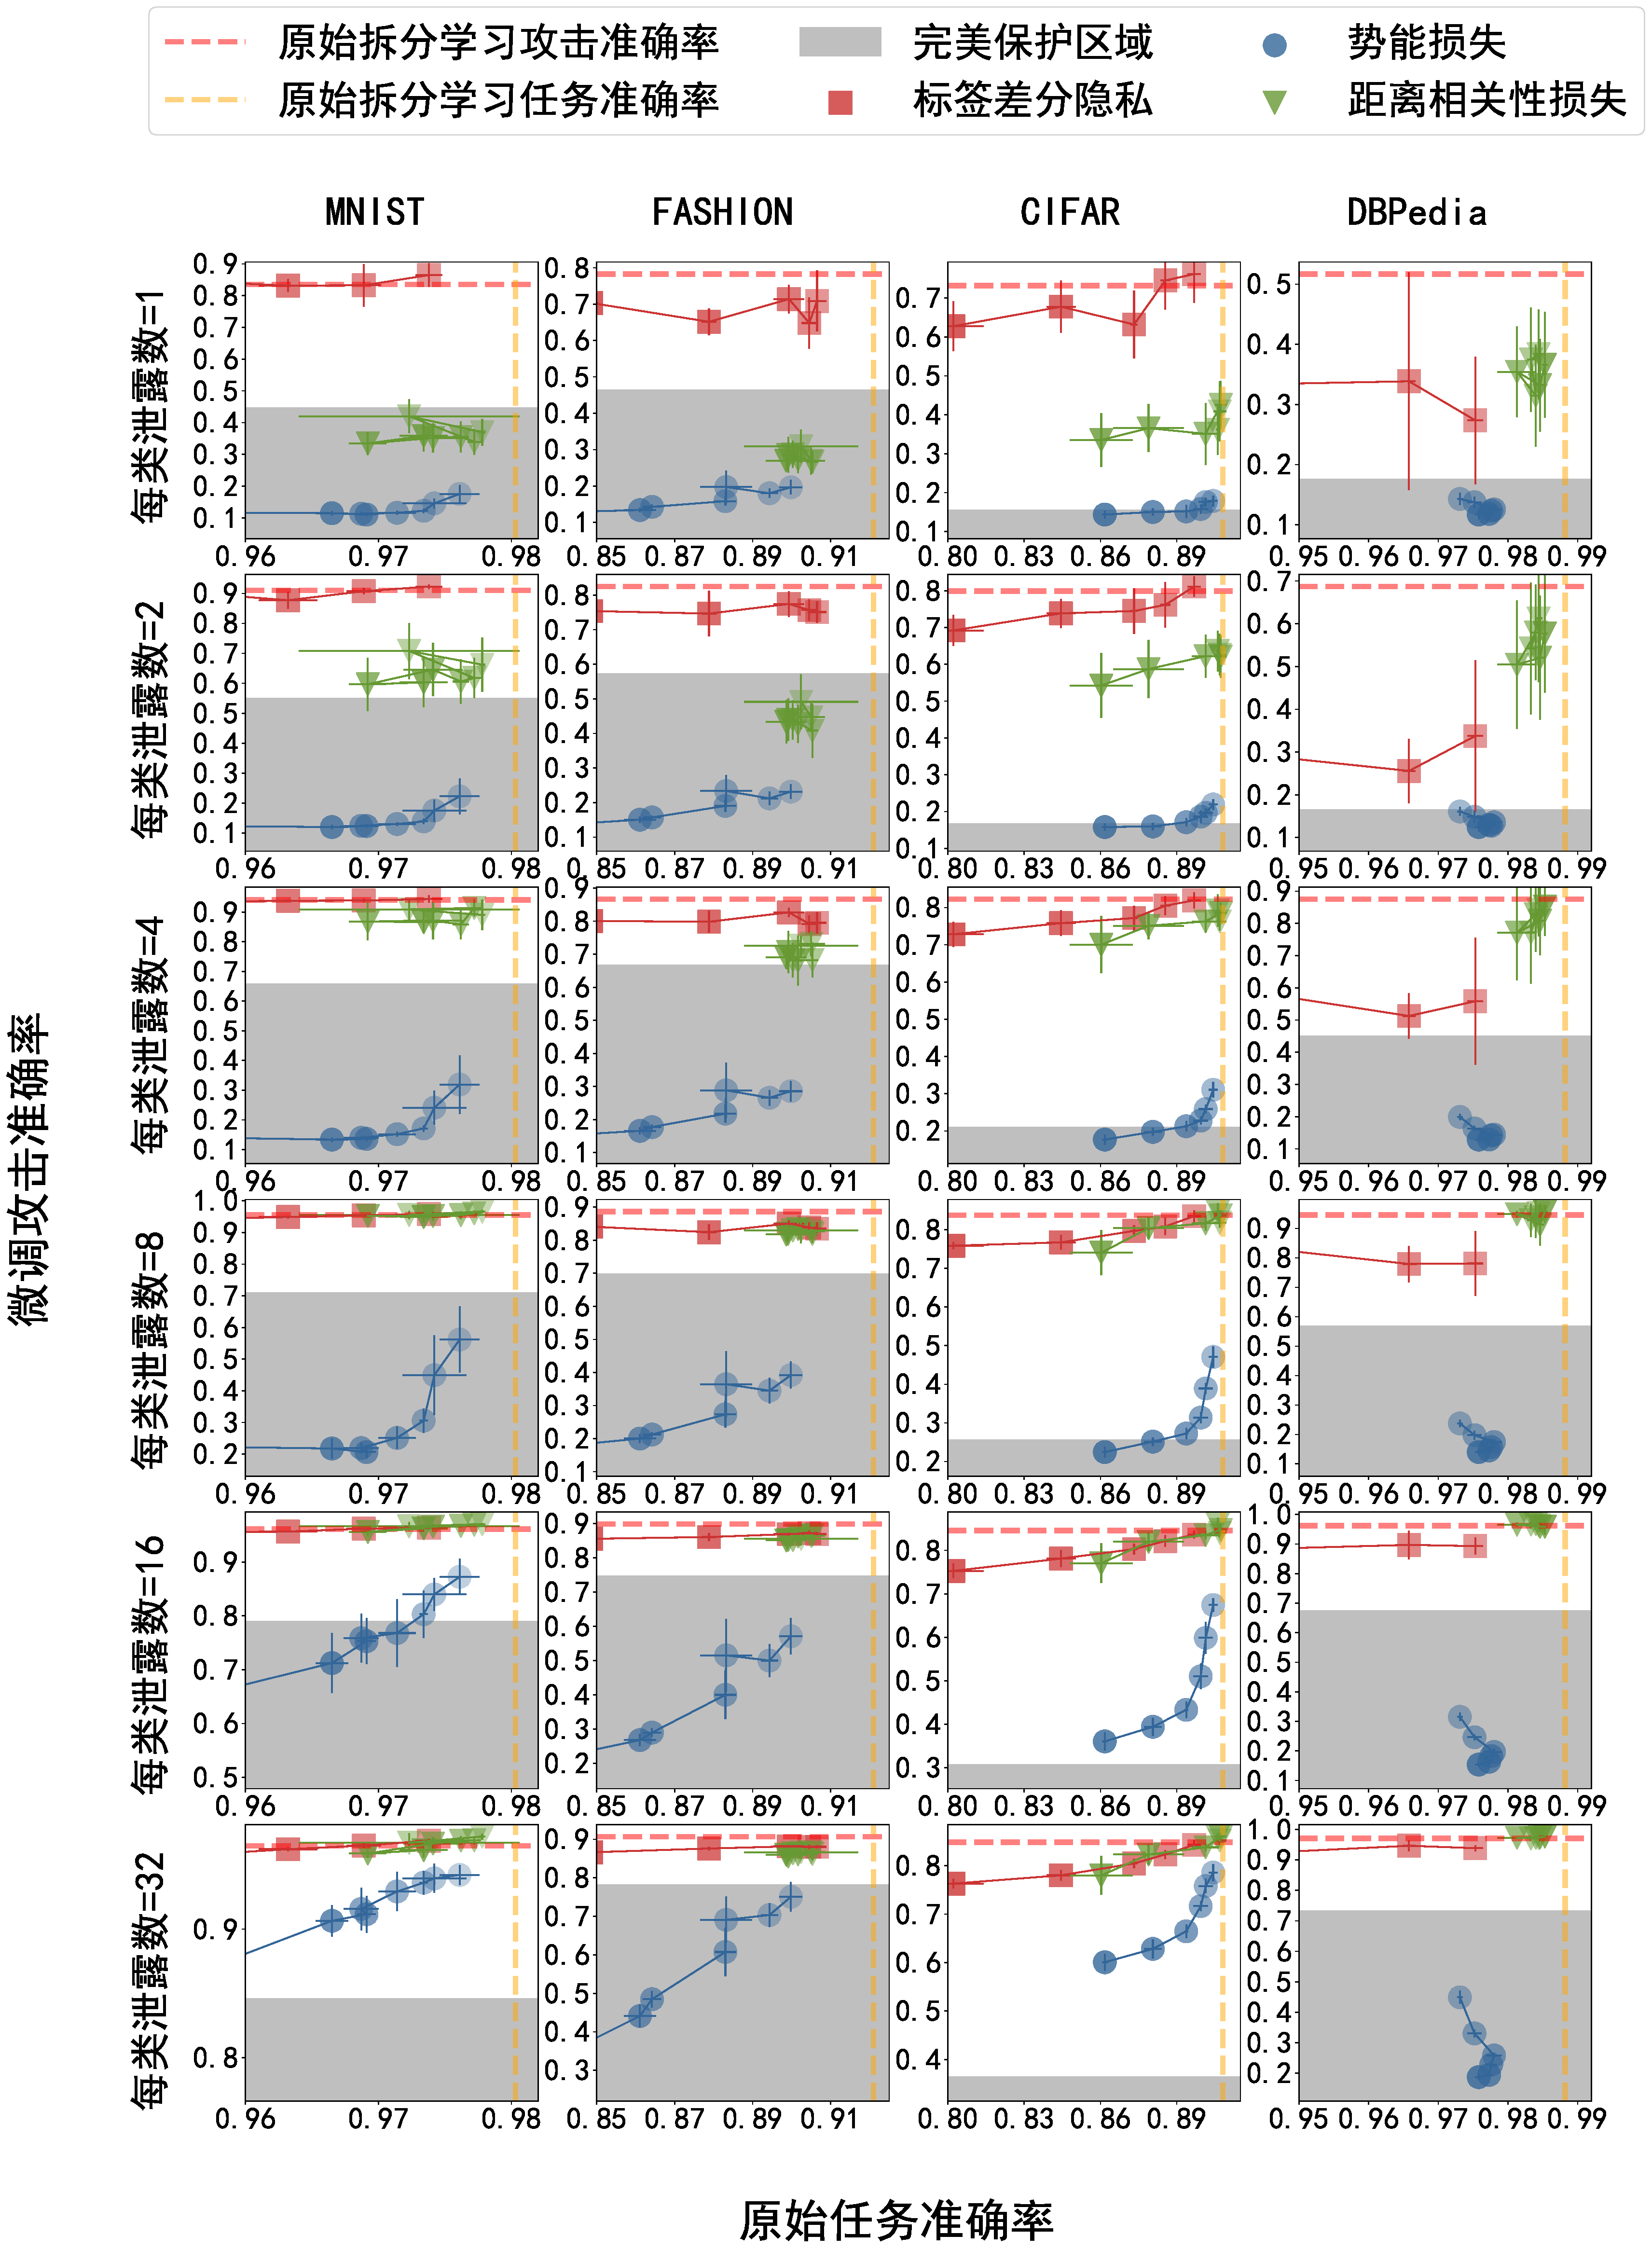
\includegraphics[width=1\linewidth]{Z_Resources/peloss_fine-tuning}
    \caption{拆分层为最后一层时原始任务准确率与微调攻击准确率对比图}
    \label{fig:peloss:fine-tuning}
\end{figure}


\begin{figure}[h!]
    \centering
    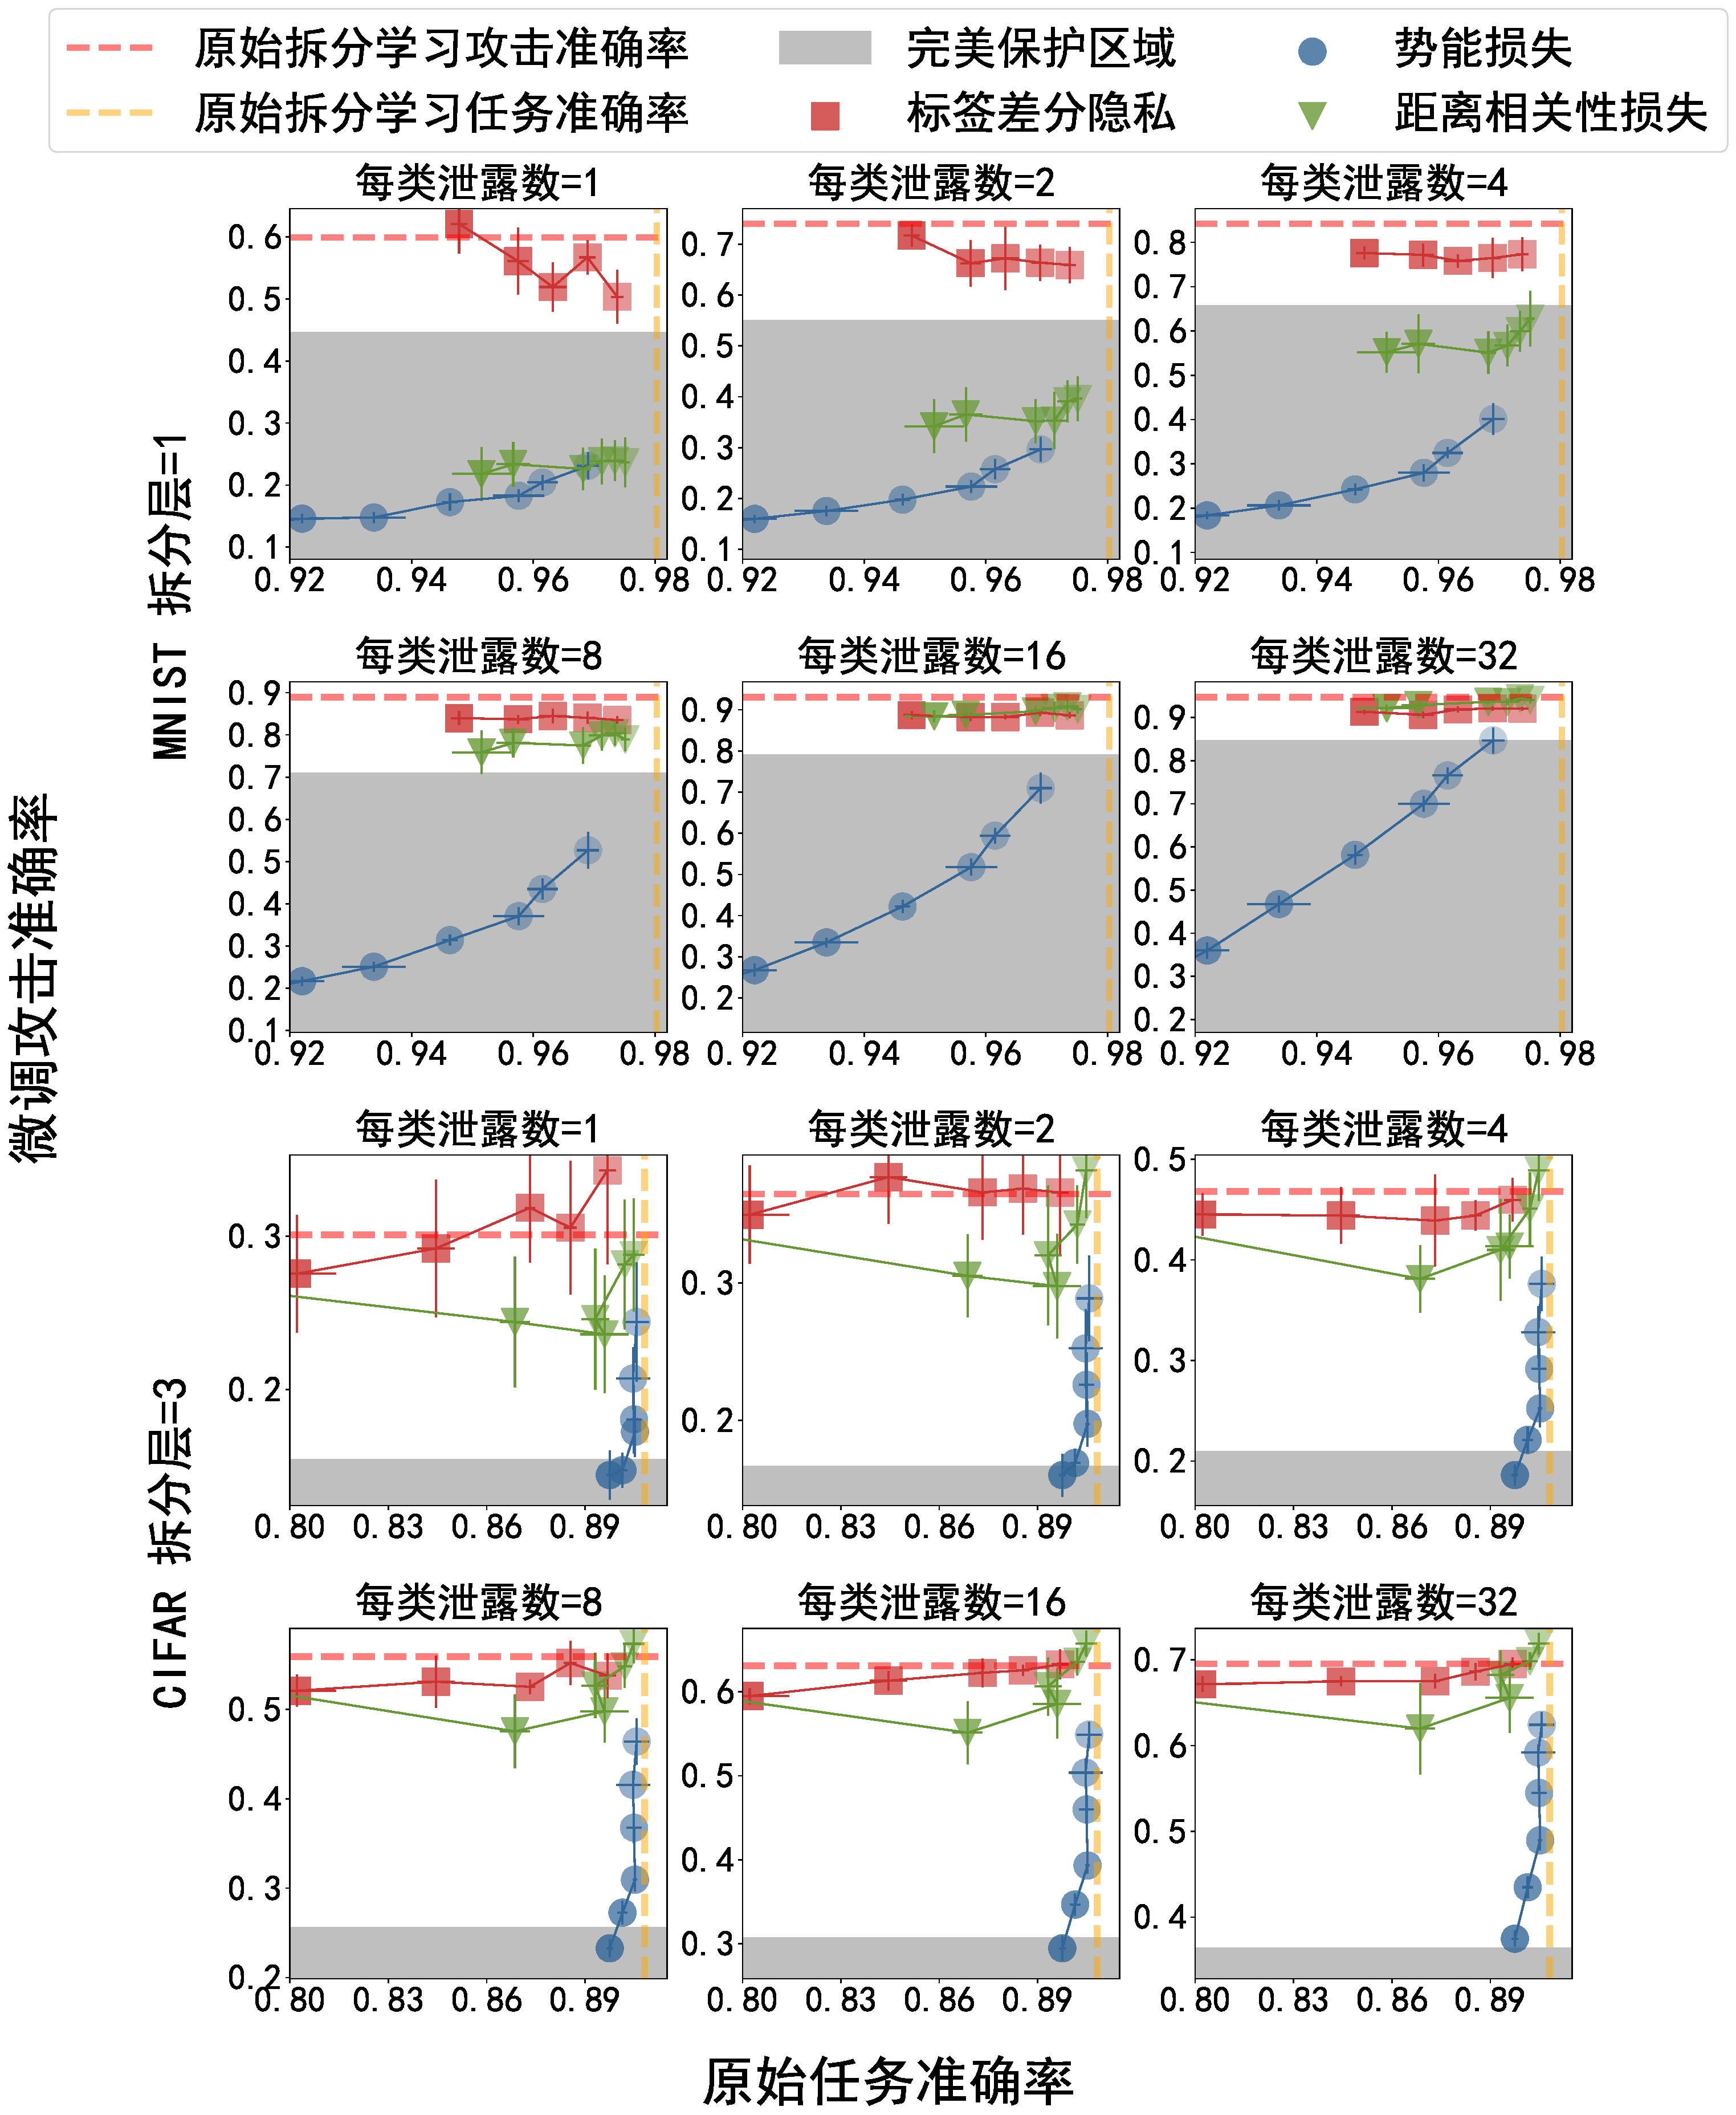
\includegraphics[width=0.85\linewidth]{Z_Resources/peloss_fine-tuning-middle}
    \caption{拆分层为中间层时原始任务准确率与微调攻击准确率对比图}
    \label{fig:peloss:fine-tuning-middle}
\end{figure}


\subsection{聚类攻击}
\begin{figure}[h!]
    \centering
    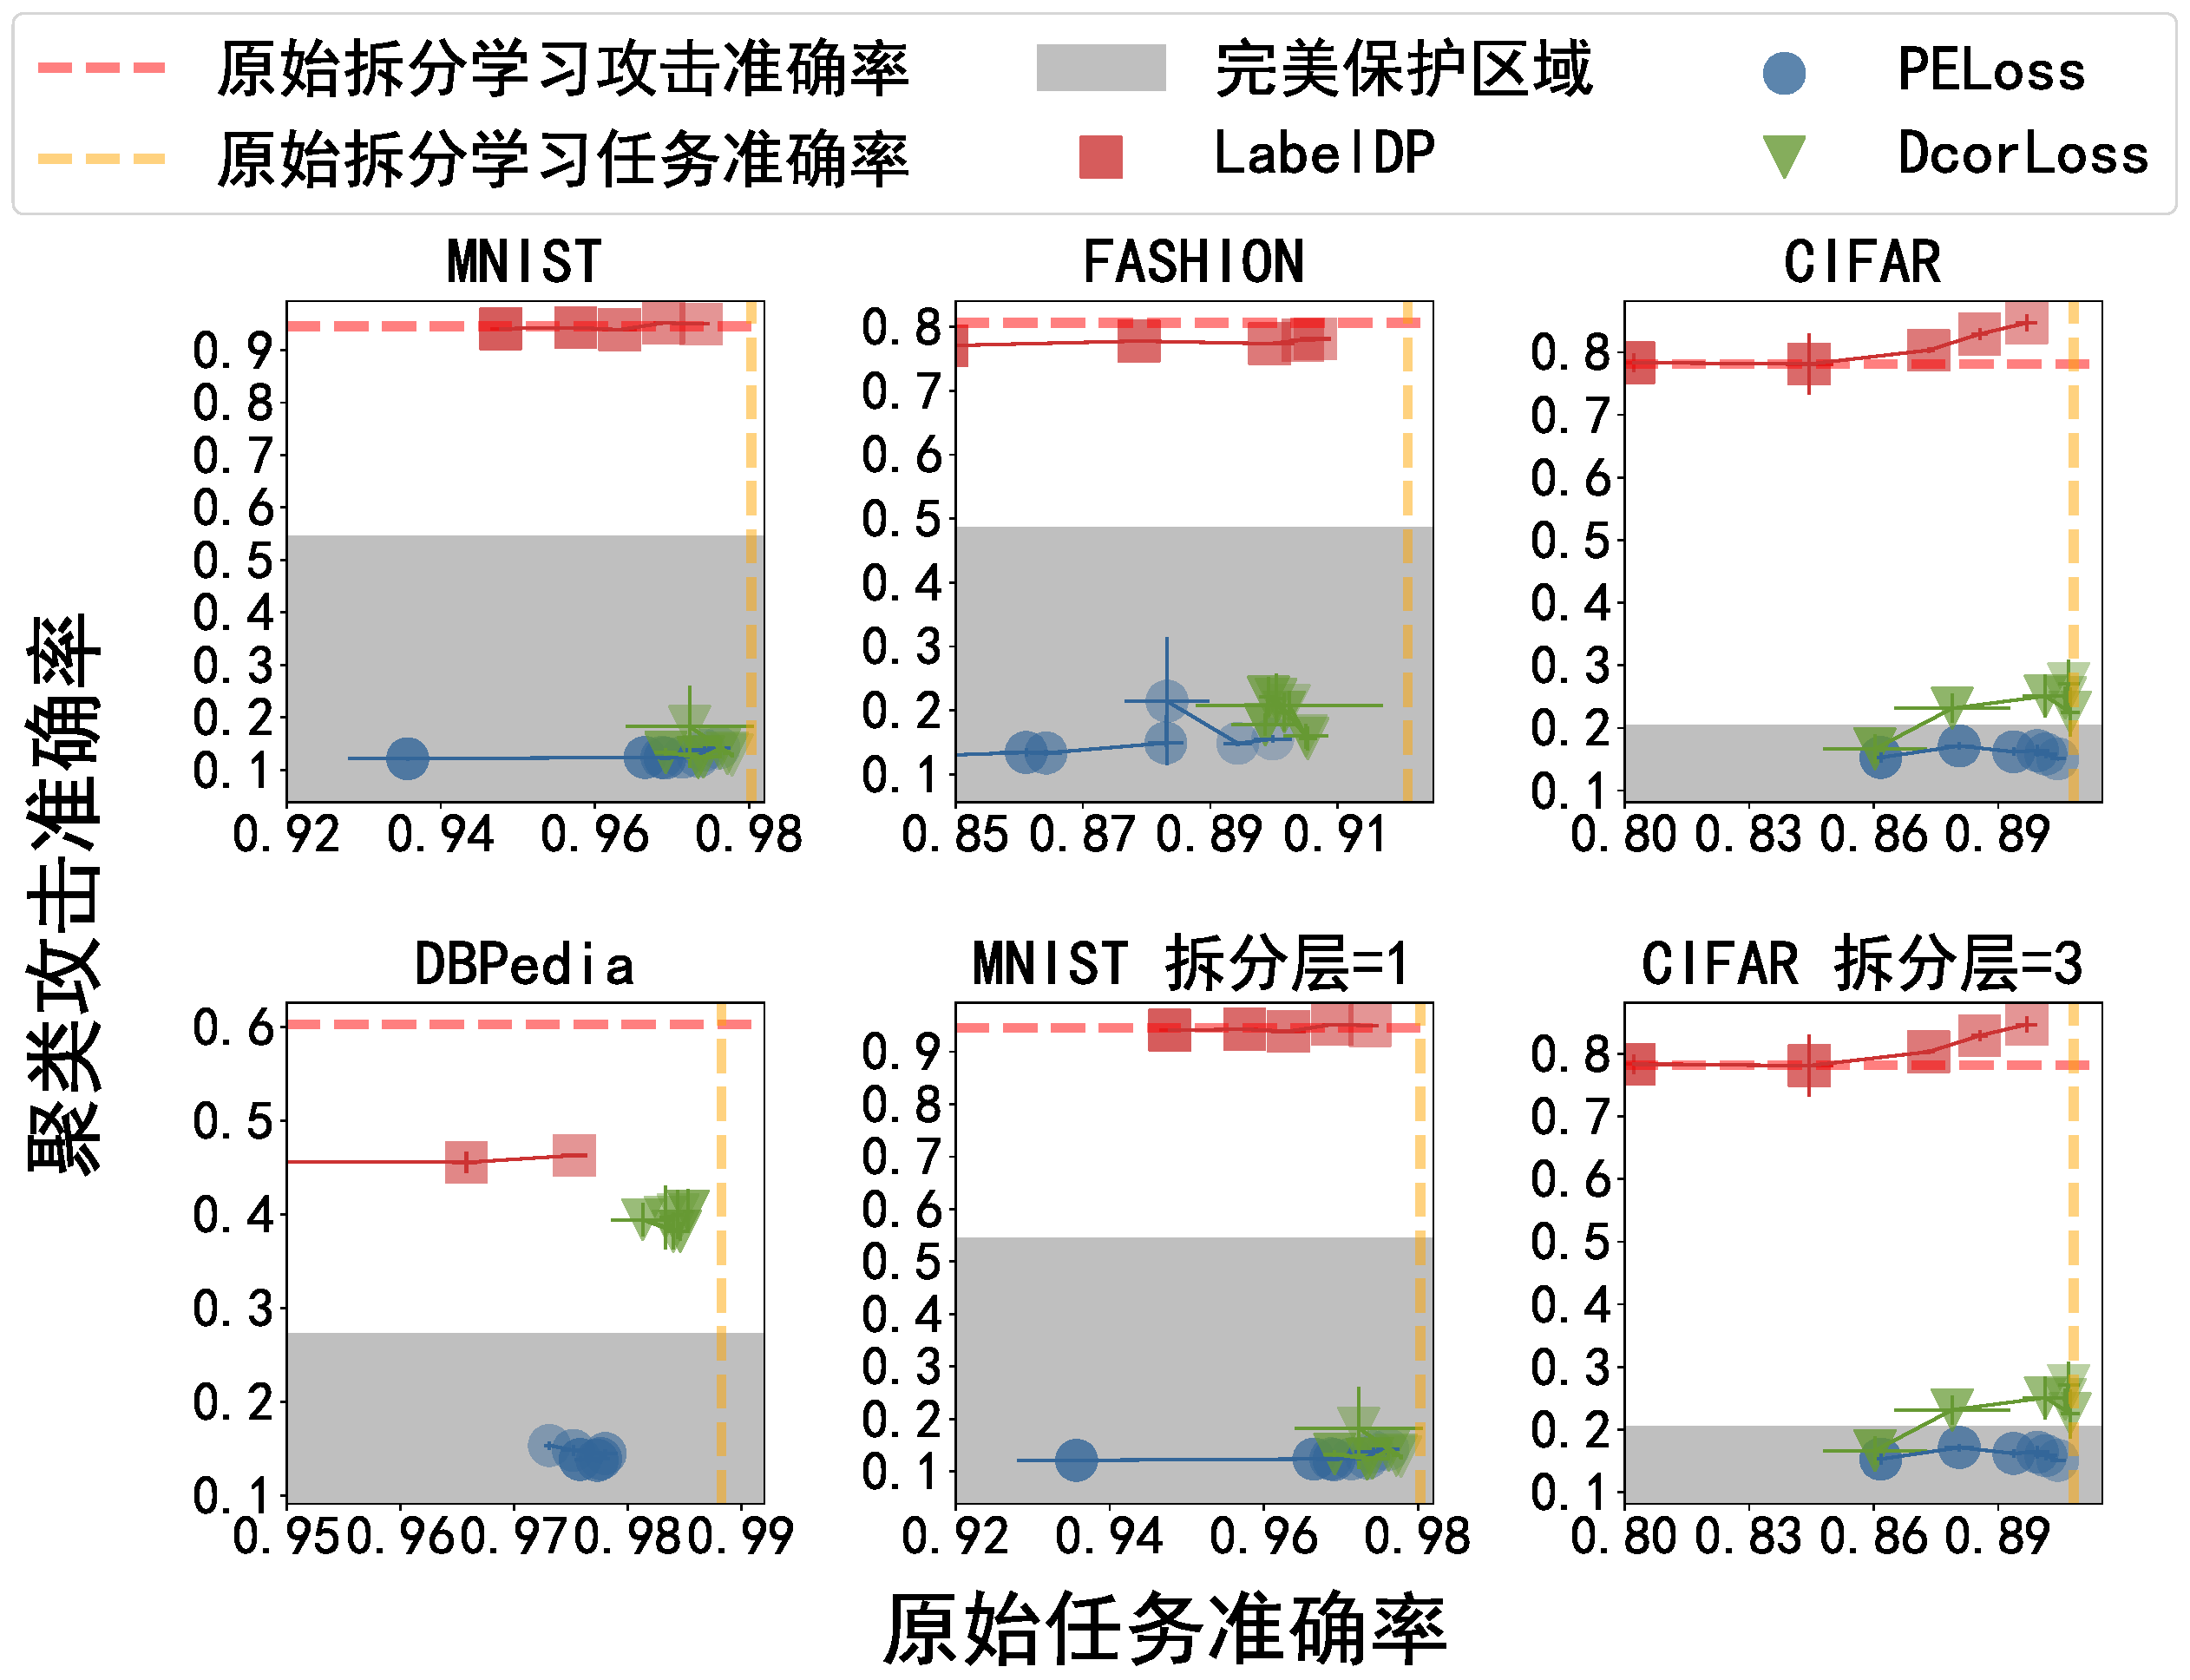
\includegraphics[width=0.8\linewidth]{Z_Resources/peloss_cluster-attack-both}
    \caption{原始任务准确率与聚类攻击准确率对比图}
    \label{fig:peloss:clustering}
\end{figure}

我们测量了模型在测试集上的准确率,以及攻击者无标签数据(整个测试集,均超过1万个样本)上进行聚类攻击得到的模型的准确率。
全部结果汇报在\autoref{fig:peloss:clustering}中。
%
由于聚类结果本身并不与实际的标签类别相对应,我们通过匈牙利匹配算法(Hungarian Matching Algorithm)~\cite{kuhn_1955_hungarian}找到准确率最高的类别映射关系并汇报该准确率。
该准确率计算公式可以表示为:
\begin{equation}
    \max\limits_{k_1,\cdots,k_C \in \text{Permutation}(1,\cdots,C)} \dfrac{\sum_{i=1}^C c_{i,k_i}}{\sum_{i,j=1}^C c_{i,j}},
\end{equation}
其中 $C$表示样本总数,$c_{i,j}$ 表示第 $i$ 个簇中实际标签是 $j$ 的样本数量, $1 < i, j \le C$。

%
实验结果表明,势能损失在所有的情况下均实现了完美保护,大幅领先于其他对比方法。
也就是说攻击者直接在泄漏的无标签数据上聚类得到的效果高于在拆分层表征上聚类得到的效果。
%
而标签差分隐私在对抗聚类攻击上效果不佳,相比于原始的拆分学习,未呈现出明显的保护作用。


\subsection{在拆分层之前攻击}
\begin{figure}[h!]
    \centering
    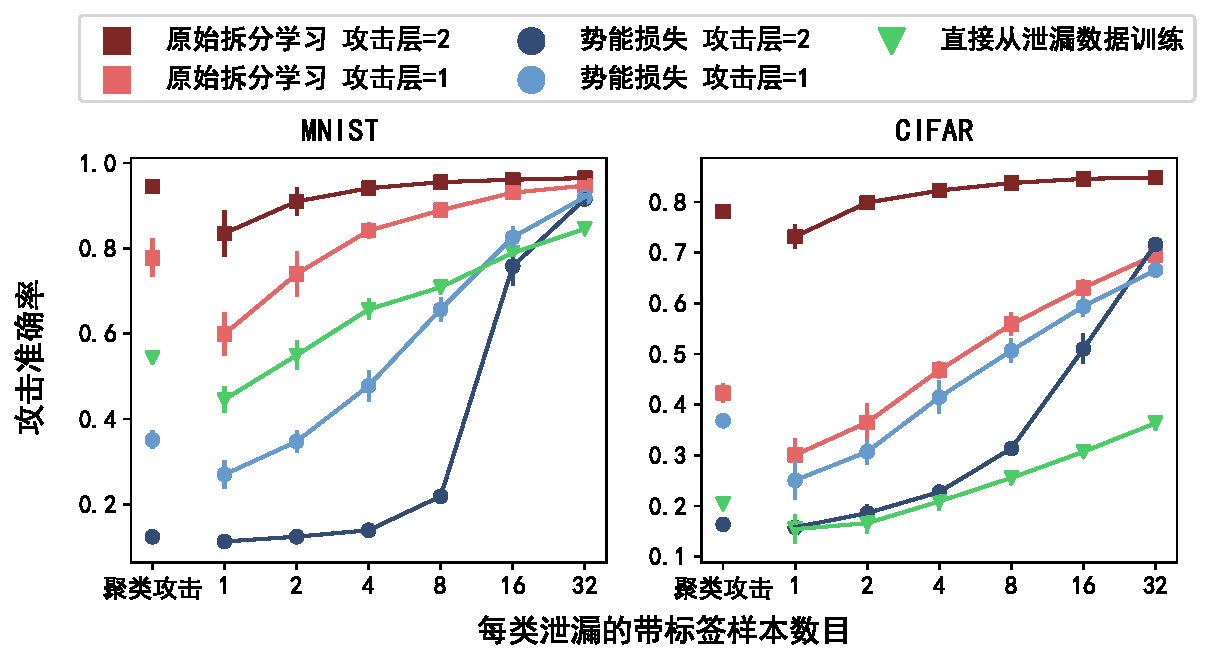
\includegraphics[width=0.85\linewidth]{Z_Resources/peloss_attack-layer}
    \caption{攻击层在拆分层之前时原始任务准确率与模型补全攻击准确率对比图}
    \label{fig:peloss:attack-layer}
\end{figure}

在之前的模型补全攻击实验中,我们假设攻击者使用了拆分层的表征进行攻击。
如果攻击者可以获取并操纵整个底部模型,则他也可以在拆分层之前的层进行攻击,也就是获取拆分层之前的隐层表征来微调模型或聚类。
%
因此,我们在MNIST和CIFAR任务中考察了攻击者在拆分层之前的层攻击的情况。
我们将拆分层设置为模型最后一个隐层,然后将MNIST任务的攻击层设置在第一个隐层处,将CIFAR-10任务的攻击层设置在第二个残差块(Residual Block)之后。
%
对于该实验,势能损失的系数被选取为$\alpha=4$。
%
我们在\autoref{fig:peloss:attack-layer}呈现在拆分层之前攻击的实验结果。

可以看到,在拆分层之前攻击可以让攻击效果有所提升,但是依然比无保护的拆分学习的攻击效果要低很多。
%
这是由于势能损失在训练过程中作用于拆分层的表征上而非之前的表征,因此拆分层之前的层的表征分布可能与标签关联性更大,使得攻击者更容易对其进行训练。

\subsection{拆分层维度的影响}
\begin{figure}[h!]
    \centering
    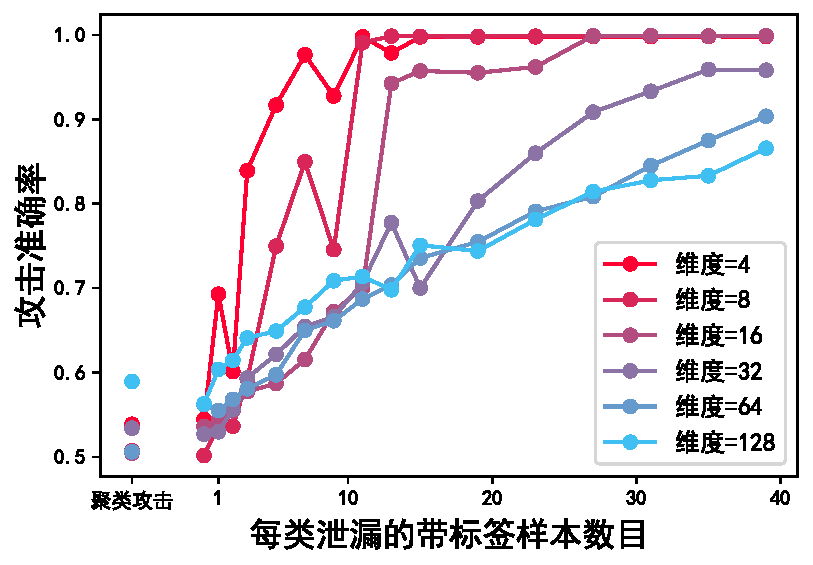
\includegraphics[width=0.7\linewidth]{Z_Resources/peloss_mnist-subclass2}
    \caption{拆分层维度对模型补全攻击准确率的影响}
    \label{fig:peloss:bottom_dim}
\end{figure}

为了研究拆分层的维度对于攻击效果的影响,我们对MNIST数据集的01子集上(只保留0和1类别的样本)进行了实验,其结果被汇报在\autoref{fig:peloss:bottom_dim}中。
此时我们设置势能损失的系数$\alpha=1$。

从图中可以看出,较高的拆分层维度大体上让微调攻击变得更难了,特别在每类样本泄露数较多的情况下。
%
例如,拆分层仅仅为4维的时候,只需要每个类别10个样本就可以让攻击准确率达到100;
而拆分层维度为128时,每类泄露40个样本后攻击准确率也不到90\%。
这是因为对更高维度的数据(也就是隐层表征)进行分类时,自然需要更多的样本。
%
作为对比,在聚类攻击时,更高的拆分层维度并未降低攻击的效果,甚至反倒有所提高。
这可能与聚类攻击时样本数量庞大有关。



\subsection{拆分层表征分布分析}
%
为了分析拆分层表征的分布,我们在MNIST数据集上计算了同类别表征之间和不同类别表征之间的角距离的分布,并且呈现在\autoref{fig:peloss:angular-distance} 中。
%
对于势能损失和距离相关性损失,我们分别把系数设置为$\alpha=1$和$\alpha=0.5$,这两者的原始任务效果基本相同。
%
图中可以看出,无论是否是同类别,抑或是属于训练集或者测试集,势能损失方法的样本表征间的角距离都接近$\pi/2$。
也就是说,无论两个表征是异类的或是同类的表征,它们都几乎相互正交。
%
对于距离相关性损失, 角距离则呈现出一个双峰分布,峰值靠近$0$和$\pi$。
并且同类别的样本表征对的角距离在靠近0的分布明显增加,导致保护效果变差。
%
而原始拆分学习中,同类别的表征之间的角距离则明显小于不同类别的表征之间的角距离,因此攻击准确率较高。


\begin{figure}[h!]
    \centering
    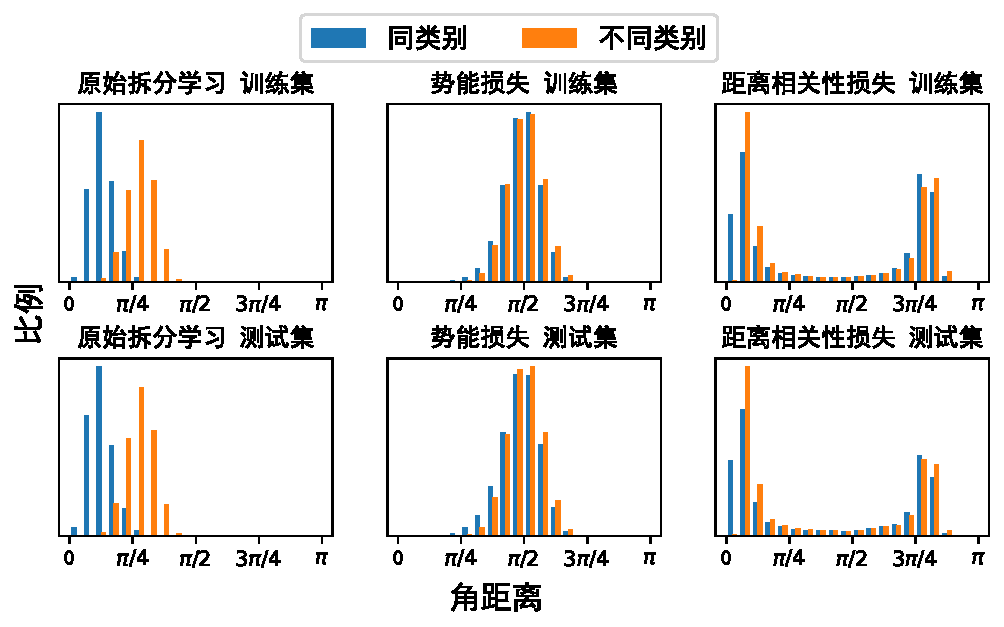
\includegraphics[width=0.8\linewidth]{Z_Resources/peloss_angular-distance}
    \caption{同类别和不同类别的隐层表征之间的角距离分布}
    \label{fig:peloss:angular-distance}
\end{figure}

为了更直观地呈现拆分层表征的分布,我们使用了t-SNE降维~\cite{van_2008_tsne}对拆分层表征进行可视化,呈现在\autoref{fig:peloss:tsne}中。
%
可以看到,原始拆分学习的拆分层表征呈现出明显的聚类性质,各个类别之间的表征可以很容易地被划分开。
%
而加入了势能损失后,不同类别的表征的分布的t-SNE投影融为一体,难以区分。
%
而距离相关性损失则呈现出了较为奇怪的分布,其分布被分为多个小块,而每个小块内都对应某个类别,且单个类别可能对应多个块。
由于同类表征间仍有一定程度的集聚效应,因此其安全性低于势能损失。

\begin{figure}[h!]
    \centering
    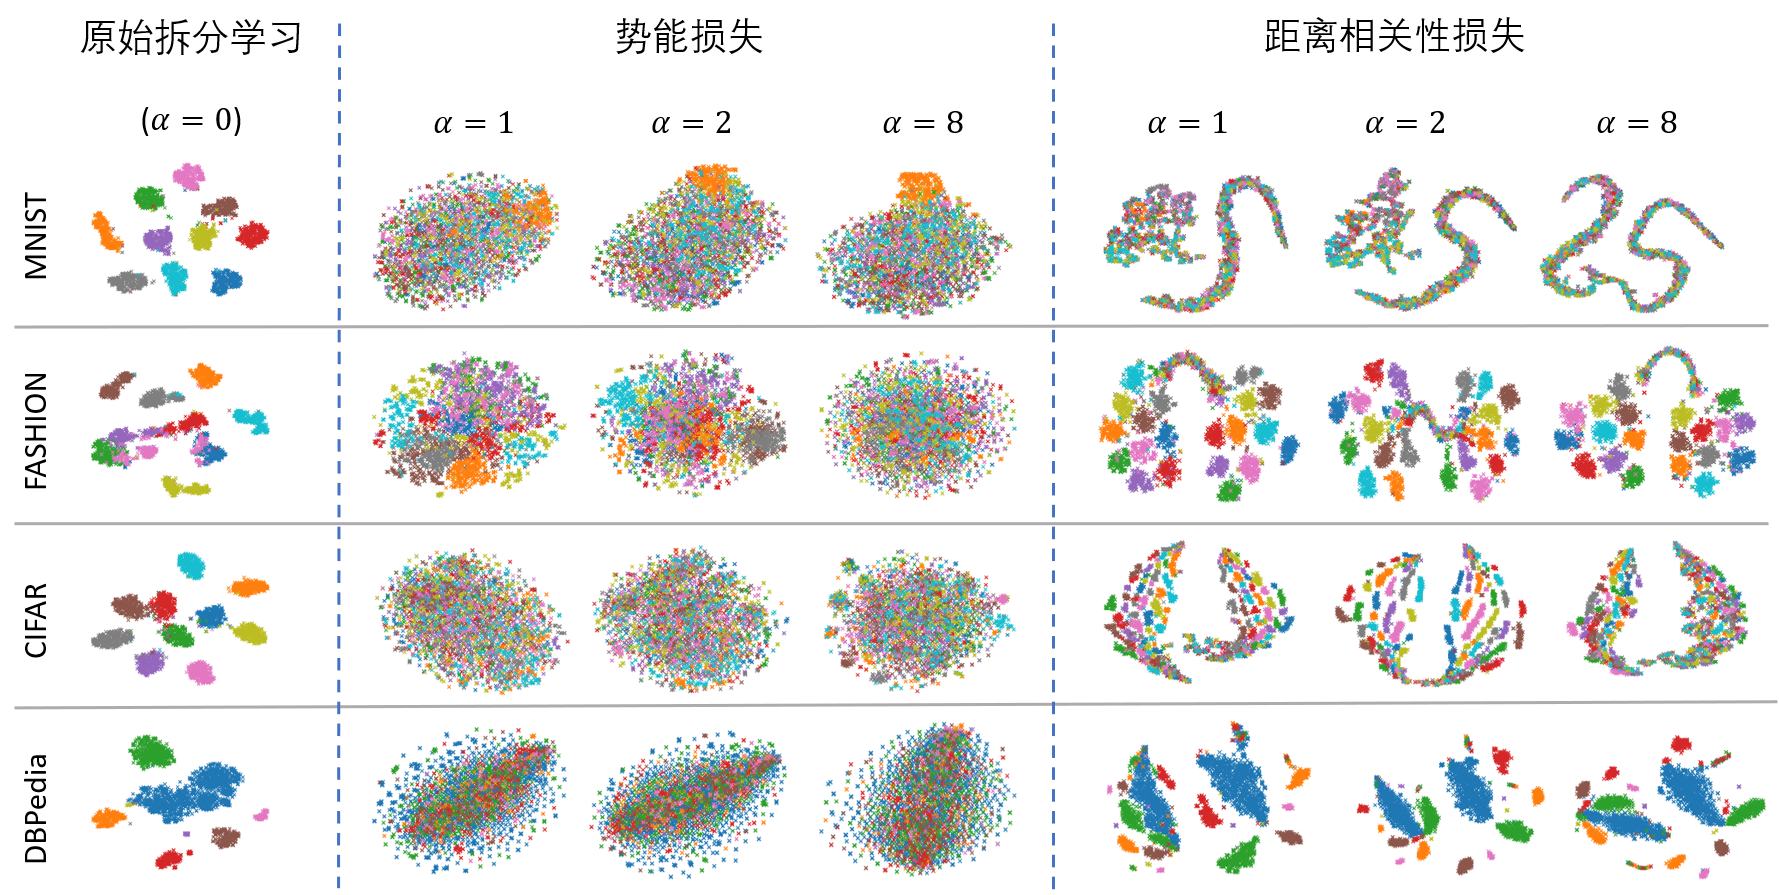
\includegraphics[width=1\linewidth]{Z_Resources/peloss_tsne}
    \caption{势能损失和距离相关性损失的隐层分布t-SNE降维}
    \label{fig:peloss:tsne}
\end{figure}


\subsection{在Transformer架构模型上的补充实验}
\begin{figure}[h!]
    \centering
    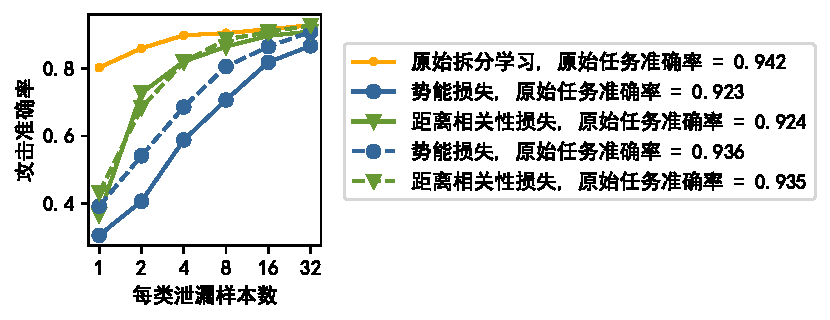
\includegraphics[width=1\linewidth]{Z_Resources/peloss_vegetable-primary}
    \caption{Vegetable Images数据集下不同泄露样本数和攻击准确率的对比}
    \label{fig:peloss:vegetable}
\end{figure}
为了进一步验证势能损失在Transformer结构的模型上的效果,我们在蔬菜图像~\cite{vegetable_2021}数据集上使用视觉Transformer(ViT, Vision Transformer)模型~\cite{alexey_2021_vit}进行了部分实验。
%
蔬菜图像数据集包含21000张图片,分为15个类别,其图片大小为$128\times 128 \times 3$。
%
我们将ViT模型的分块大小(Patch Size)设置为$16\times 16$,隐层大小为256,层数为4,注意力头(Attention Heads)个数为8。
%
实验结果呈现在\autoref{fig:peloss:vegetable}中,可以看出,势能损失在ViT模型上依然显著领先于对比的距离相关性损失。
\section{本章小结}
本章节针对拆分学习模型推断过程中的标签隐私泄露以及模型补全攻击问题,提出了受物理学现象启发的势能损失函数。
%
我们将模型补全攻击转化成一个攻击者的有监督或无监督的学习问题,通过分析泛化误差、聚类误差,表明拆分层表征分布在决策区域边缘可以增加攻击者的攻击难度,而势能损失函数恰好可以帮助样本的拆分层表征产生如此分布。
%
实验结果表明,势能损失函数在多个数据集、不同的泄漏标签数量上均优于对比算法,同时保证了原始任务准确率和攻击误差。
%
总之,势能损失降低了拆分学习推断过程中的隐私泄露问题,为拆分学习模型的实际应用提供了有力保护。